\chapter{Future Work}
Code generation using TEBNF creates several possibilities for future work.  The first possibility is to add more I/O methods to TEBNF and the TEBNF code generation tool.  There are many different ways to receive input and send output beyond what is currently supported by TEBNF and the TEBNF code generation tool.  Another possibility involves the creation of an integrated development environment for TEBNF.  The last improvement covered in this chapter is to add support into the TEBNF code generation tool to automatically generate graphical user interfaces at runtime.

\section{New I/O Methods}
A wide range of I/O methods could be added to TEBNF.  This could include adding support for interacting with relational databases.  Support for commonly used database query languages like MySQL and PostgreSQL would allow TEBNF to interact with a wide range of systems that utilize databases.

\indent
The TCP/IP protocol is widely used and could be adapted into a set of I/O methods.  Due to the fact that TCP/IP is connection-oriented, I/O methods would be needed that support both server and client I/O.

\section{Integrated Development Environment}
A TEBNF Integrated Development Environment (IDE) could provide intelligent code completion or incorporate a drag-and-drop interface for adding TEBNF elements to a grammar.  The IDE could also support GUI design.

\section{Runtime Graphical User Interface Generation}
Support for automatic GUI generation could be integrated into the TEBNF code generation tool.  Console user interfaces for generated applications would be replaced with a web-based GUI that communicates with the generated application.  The code generation process would need to employ a runtime data mining technique called software mining \cite{kennard_01,kennard_02}, which is a form of data mining that focuses on the inspection of static and runtime software information characteristics.  Some examples of static characteristics include source code files and database schemas, while runtime characteristics include polymorphic data-types, data values, and the reading and modification of an instantiated object’s current state.

\indent
Software mining would take place during all phases of the TEBNF code generation process, beginning with lexical analysis.  Static characteristics including element and subelement names would be gleaned from tokens as they are read from the input grammar by the TEBNF scanner.  During the syntactic analysis phase, static characteristics observed from the lexical analysis phase help to identify which runtime characteristics from the parse tree should be used to map element objects and subelement objects to their appropriate GUI controls.  This mapping would consist of annotations added to each element and subelement object in the parse tree.  These annotations would describe which attributes require GUI interaction and how this interaction is linked to the data being handled by the code.
Next, the TEBNF resolver traverses the parse tree in order to resolve all elements and subelements.  While traversing the tree, annotations from the syntactic analysis phase are analyzed in order to select the appropriate control(s) for the GUI.  Information about the GUI control(s) and how they link to data being handled by that element or subelement is added to the annotations.

\begin{figure}[h!]
\centering
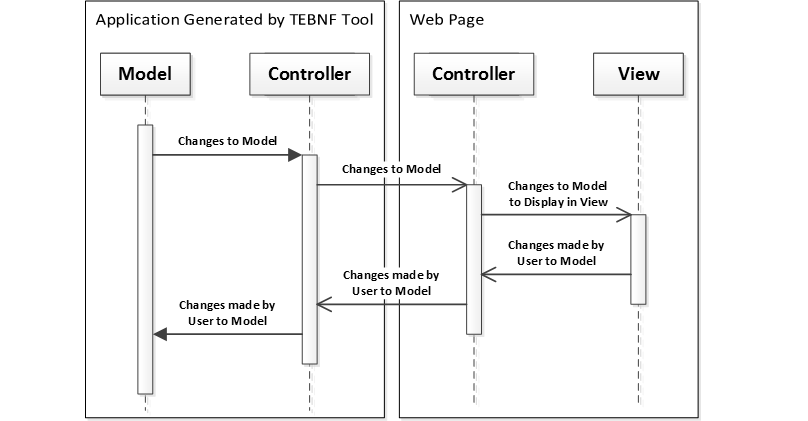
\includegraphics[width=0.9\textwidth]{figures/DmvcCommSequence.png}
\caption{DMVC communication sequence between an application and GUI generated by the TEBNF code generation tool.}
\label{fig:DmvcCommSequence}
\end{figure}

\indent
Code for the GUI would then be generated during the code generation phase.  Generated GUI code follows a form of the Model-View-Controller (MVC) design pattern called Dual-MVC (DMVC) \cite{leff_01}.  The generated executable contains the actual Model and a Controller.  A web page contains another Controller and the View (GUI).  Because the web page represents the state of the application, it contains a partial representation of the Model.  Changes to the View are sent to the web page Controller.  Those changes are sent from the web page Controller to the executable Controller which then conveys those changes to the Model as needed.  Changes to the Model can cause changes that need to be reflected in the View.  The Model can send those changes to the executable’s Controller.  It then sends the changes back up to the web page Controller which updates the View.  Figure~\ref{fig:DmvcCommSequence} illustrates how communication between an application generated by the TEBNF code generation tool and its GUI would be deployed under the DMVC architecture.

\begin{figure}[h!]
\centering
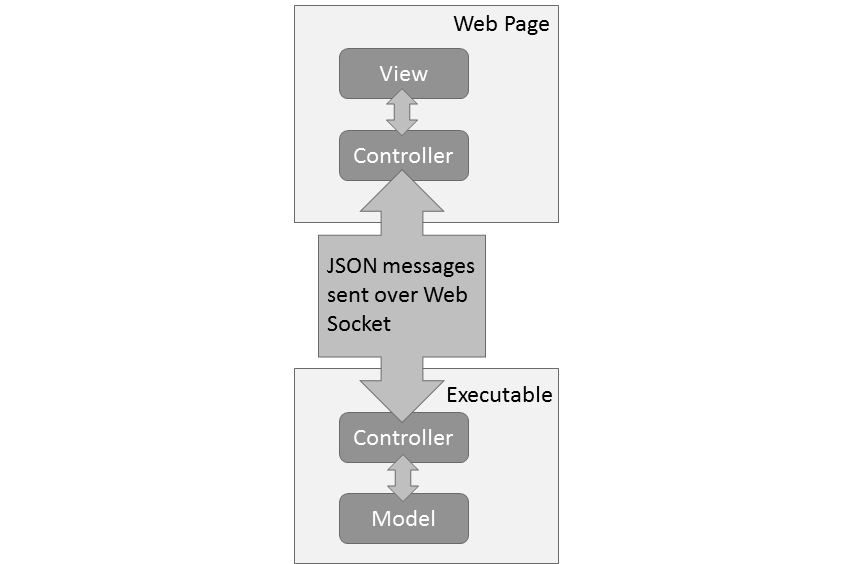
\includegraphics[width=0.9\textwidth]{figures/DmvcStructure.png}
\caption{DMVC structure of an application and GUI generated by the TEBNF code generation tool.}
\label{fig:DmvcStructure}
\end{figure}

\indent
Annotations from the parse tree are used to create JSON messages to be sent from the generated application Controller to the web page Controller.  These JSON messages contain information representing widgets and their layouts on the web page.  The web page Controller receives these JSON messages directly from the generated application via a HTML5 web socket.  The connection and maintenance of this web socket is managed by both of these controllers.  The mapping of objects to widgets on the application side using JSON messages is the first of a two stage Object User Interface Mapping (OIM) process.

\indent
These JSON messages make it easier for the web page Controller to perform the second OIM stage.  This involves conversion of JSON messages received over a web socket connection into GUI widgets along with their layouts.

\indent
Changes made by the user in the web page GUI View are sent back to the application over the same web socket as JSON messages (figure~\ref{fig:DmvcStructure}).  These JSON messages contain the current state of the web page View along with any changes to it made by the user.
